\documentclass[11pt,twocolumn]{article} 
\usepackage{geometry}
\usepackage{bm}
% \geometry{left=2cm,right=2cm,top=1cm,bottom=2cm}
\usepackage{simpleConference}
\usepackage{times}
\usepackage{graphicx}
\usepackage{amssymb}
\usepackage{url,hyperref}

\usepackage{booktabs} 
\usepackage{amsfonts}  
\usepackage{amsmath}
\usepackage{float}
\usepackage{subfigure}
\usepackage{setspace}
\renewcommand{\baselinestretch}{1.0}

\usepackage[sort]{natbib}  % 引文格式
\usepackage{multicol}
\usepackage{multirow}
\usepackage{setspace} % 可设置表格行高
% \usepackage[colorlinks, linkcolor=blue]{hyperref} % 超链接
\usepackage{float} %图片紧跟文字
\usepackage{subfigure}
% set page geometry
% \usepackage[verbose=true,letterpaper]{geometry}
\AtBeginDocument{
  \newgeometry{
    textheight=9in,
    textwidth=6.8in,
    top=1in,
    headheight=14pt,
    headsep=25pt,
    footskip=30pt
  }
}

% \widowpenalty=10000
% \clubpenalty=10000
% \flushbottom
% \sloppy

\usepackage{fancyhdr}
\pagestyle{fancy}
\lhead{} 
\rhead{} 
\chead{\bfseries CIE6036 Project Results} % CIE6036 Project Report
% \lfoot{} 
\cfoot{\thepage}
% \rfoot{\thepage} 
\renewcommand{\headrulewidth}{0.4pt} 
% \renewcommand{\footrulewidth}{0.4pt}
\usepackage[font=small,labelfont=bf]{caption}


\begin{document}

\title{Decision Making of Dynamic Airlines System under Epidemic Environment}

\author{Yu Fangchen, Cai Weilin, Li Chi, Chen Weibin \\
	\and
	Department of Computer and Information Engineering\\
	The Chinese University of Hong Kong, Shenzhen \\ \\
	\today
}

% \author{Yu Fangchen \\
% 	\texttt{220019040@link.cuhk.edu.cn} \\
% 	\and
% 	Cai Weilin \\
% 	\texttt{220019066@link.cuhk.edu.cn} \\
% 	\and
% 	Li Chi \\
% 	\texttt{220019044@link.cuhk.edu.cn} \\
% 	\and
% 	Chen Weibin \\
% 	\texttt{220019062@link.cuhk.edu.cn} \\
% 	\and
% 	Department of Computer and Information Engineering\\
% 	The Chinese University of Hong Kong, Shenzhen \\ \\
% 	\today
% }

\maketitle

\small


\begin{abstract}
% TODO Change Dynamic Programming into other expression (important) .
Inspired by the fusing command from civil aviation, the decision making of dynamic airline system takes a more essential role in current situation. Firstly, we propose a new decision making model on airline capacity and formulate a constrained optimization problem. After the problem is mathematically simplified into linear constraints, we apply the Differential Evolution Algorithm to obtain the optimal decisions. The empirical experiments shows the necessity to greatly reduce the capacity of airline from the cities with severe outbreaks, which demonstrates excellent potential in broader application\footnote{Codes: \url{github.com/WhiskyChoy/NwEcoPrj}}.
\end{abstract}

% \keywords{Network Economics, Dynamic Programming, Infection Model}

\section{Introduction}

\subsection{Choice of Project}
\emph{An original network economics research}

\subsection{Project Scenarios}

For the year 2020, people are still suffering from the COVID-19 pandemic. It brings severe challenge to the operation of traditional service industry. The aviation industry is one of those most impacted under the pandemic, since protective measures against infection could set tight restriction to the capacity of the transportation network. For example, governments around the world have prohibited cross-country transportation and the market share of the airline business has shrunk since then. Some methodologies like an event-driven approach have been implemented to quantitatively analyze the economic influence, especially after three major COVID-19 announcements were made by World Health Organization (WHO) \cite{maneenop2020impacts}. Other studies focus on scenarios variation after post-COVID-19 and how airlines react and recover from the pandemic in the aspect of world airline network (WAN) \cite{ye2020scenarios}. Aviation network features like temporal characteristics can also influence the infection rate \cite{scire2017}. Among the countries that waged arduous struggles to the pandemic, China is one of those achieved early recovery. The "Five One" policy adopted by the Civil Aviation Administration of China (CAAC)\footnote{Official website: \url{www.caac.gov.cn/en}} to prevent imported cases could play a big role. It allows mainland carriers to fly just one flight a week on one route to any other country and foreign airlines to operate just one flight a week to China. From the perspective of airline markets, some foreign airlines also make strategic response to the pandemic crisis and outline key implications for post-COVID-19 competitive landscape, to raise attention and provide recommendations for policy makers \cite{albers2020european} \cite{budd2020european}. Inspired by such fusing measures and response behavior, we further expand the decision making process into an air traffic control problem. Here we try to provide similar policies for cities in the transportation network, considering both the infection rate and passengers' utility.


\subsection{Goals}
To achieve our goals, we try to answer the following questions:
\begin{itemize}    
    \item How should we model the aviation network under the pandemic?
    \item What's the best strategy for each city/for the global network?
    \item Is there any penalty of anarchy and how do we describe it?
\end{itemize}

% \begin{itemize}
%     \item 
%     How should we model the aviation network under the pandemic? 
%     \item 
%     What's the best strategy for each city/for the global network?
%     \item
%     Is there any penalty of anarchy and how do we describe it?
% \end{itemize}

These are novel questions to solve. The solution to the first question is the foundation for our further discussion, and we try to carry out exploratory experiments seeking the solution to the second question. The third question is hard to solve and requires further distribution in such area. The main contributions of this project are the following:
\begin{itemize}
    \item We propose a new decision making model on airline capacity considering both the passengers' demand and the infection severity of different cities.
    \item We mathematically simplify our model and make it solvable under linear constraint in \emph{IBM CPLEX} solver. We also apply the Differential Evolution Algorithm using the \emph{GeatPy}\cite{geatpy} toolkit to solve our problem and find better result.
    
    \item Empirical experiments have been done to show the necessity to ban the airlines from cities with high infection severity and the difficulty to strike a balance between the demand of passengers and public health. 
\end{itemize}

The paper is organized as follows. Section 2 reviews the related work. Section 3 introduces our models, while Section 4 presents our algorithms. Section 5 reports the empirical experiments and results, followed by the discussion and conclusions in Section 6. Lastly, Section 7 briefly introduces the contributions by each group member. 
y

% =================================

\section{Related Work}
Recently, researchers have done forecasting based upon data sources received from authenticated national and international sources. Effectiveness of forecasting is based upon the quality of data source used for forecasting. Forecasting results may vary based on the impurities in the data sources. Data mining and big data techniques always play a vital role for the forecast system\cite{huang2018air}. Previously, Giulia Giordano\cite{giordano2020sidarthe} has proposed the SIDARTHE Model that helps in redefining the reproduction number. This epidemic prediction model compares the infected density with the level of symptoms. Jia Wangping\cite{wangping2020extended} has presented a study in which, COVID-19 data from Jan 22, 2020, to Mar 16, 2020, has been used in time series form for analysis. Extended susceptible-infected-removed (eSIR) model. The prediction has been estimated using the Markov Chain Monte Carlo method and results show that the reproductive number in Italy is 4.10 and 3.15 in Hunan. China has successfully used a variety of measures to control the COVID-19 such as controlling the public transportation\cite{shen2020prevention,kucharski2020early}. Based on these previous studies, we would like to use a model to solve the network flow problem of airline system for dynamic control, which might control the epidemic and bring less economic losses. 
\begin{itemize}
    \item \textbf{Network flow problem}
    Network flow is a network that satisfies the following properties. Each edge has a maximum capacity C, which is the maximum flow that the edge can accommodate. f is the actual traffic flowing through the edge, and there is always f less or equal to C.
    \item \textbf{Minimum cost maximum flow problem}
The minimum cost maximum flow problem is a typical problem in economics and management. Each path in a network is limited by cost and capacity. These kind of research problems are mainly want to find out how to select the path and allocate the traffic passing through the path from a to B can achieve the minimum cost requirement.
    \item \textbf{Susceptible-infectious (SI) model }
    SI is the most basic epidemic model. S and I are Susceptible and Infectious respectively. This model assume that the susceptible person and the Infectious person effective contact is infected with Infectious person. SI model is one of the main methods to control and prevent infectious diseases. In different cases, we can add other kind of persons like exposed person and recover person, which can better illustrate different infectious diseases.

\end{itemize}
% =================================

\section{Related Work}
Recently, researchers have done broad and in-depth studies focusing on how COVID-19 affected our daily life from the perspective of economic, culture and social behaviors. Treating the process of COVID-19 as a susceptible-infected model, Jia Wangping\cite{wangping2020extended} has presented a study in which, COVID-19 data from Jan 22, 2020, to Mar 16, 2020, has been used in time series form for spreading analysis. In the aspects of public transportation, a variety of effctive measures have been successfully implemented to control the COVID-19 \cite{shen2020prevention,kucharski2020early}. In our paper, decision making of dynamic airline rearrangement is actually a network optimization problem. Shangyao Yan \cite{yan2002passenger} develops an integer multiple commodity network model and a solution algorithm to help carriers simultaneously solve for better fleet routes and appropriate timetables. Some heuristic algorithms such as genetic algorithm \cite{kolker2015using} and dynamic programming \cite{khoo2014bi} have also beem applied to solve airline network and fleet planning problems. Based on these previous studies, we would like to use a model to solve the network flow problem of airline system for dynamic rearrangement, which might control the epidemic and bring less economic losses. 
\begin{itemize}
    \item \textbf{Network flow problem}
    Network flow is a network that satisfies the following properties. Each edge has a maximum capacity $C^{max}$, which is the maximum flow that the edge can accommodate. $C$ is the actual traffic flowing through the edge, and there is always $C$ less or equal to $C^{max}$.
    \item \textbf{Minimum cost maximum flow problem}
The minimum cost maximum flow problem is a typical problem in economics and management. Each path in a network is limited by cost and capacity. These kind of research problems are mainly want to find out how to select the path and allocate the traffic passing through the path from a to B can achieve the minimum cost requirement.
    \item \textbf{Osmosis model}
    Osmosis can be described by a phenonomenon where the spontaneous net of solvent molecules moves through a selectively permeable membrane into a region of higher concentration, in the direction that tends to equalize the two-sided solute concentration. It can also demonstrate a physical process in which any solvent moves across a selectively permeable membrane. In this way, the infection rate between two selective cities can be defined as different levels of solute concentration while flight movements will be regarded as the process of solvent molecules osmosis.   
\end{itemize}
\section{Proposed Model}

% \subsection{General Model}

Let us focus on the simplest situation. Considering a group of independent cities, we can draw a simple graph to describe the connectivity between cities, which means the direction and capacity of airlines. 
\begin{figure}[H]
    \centering
    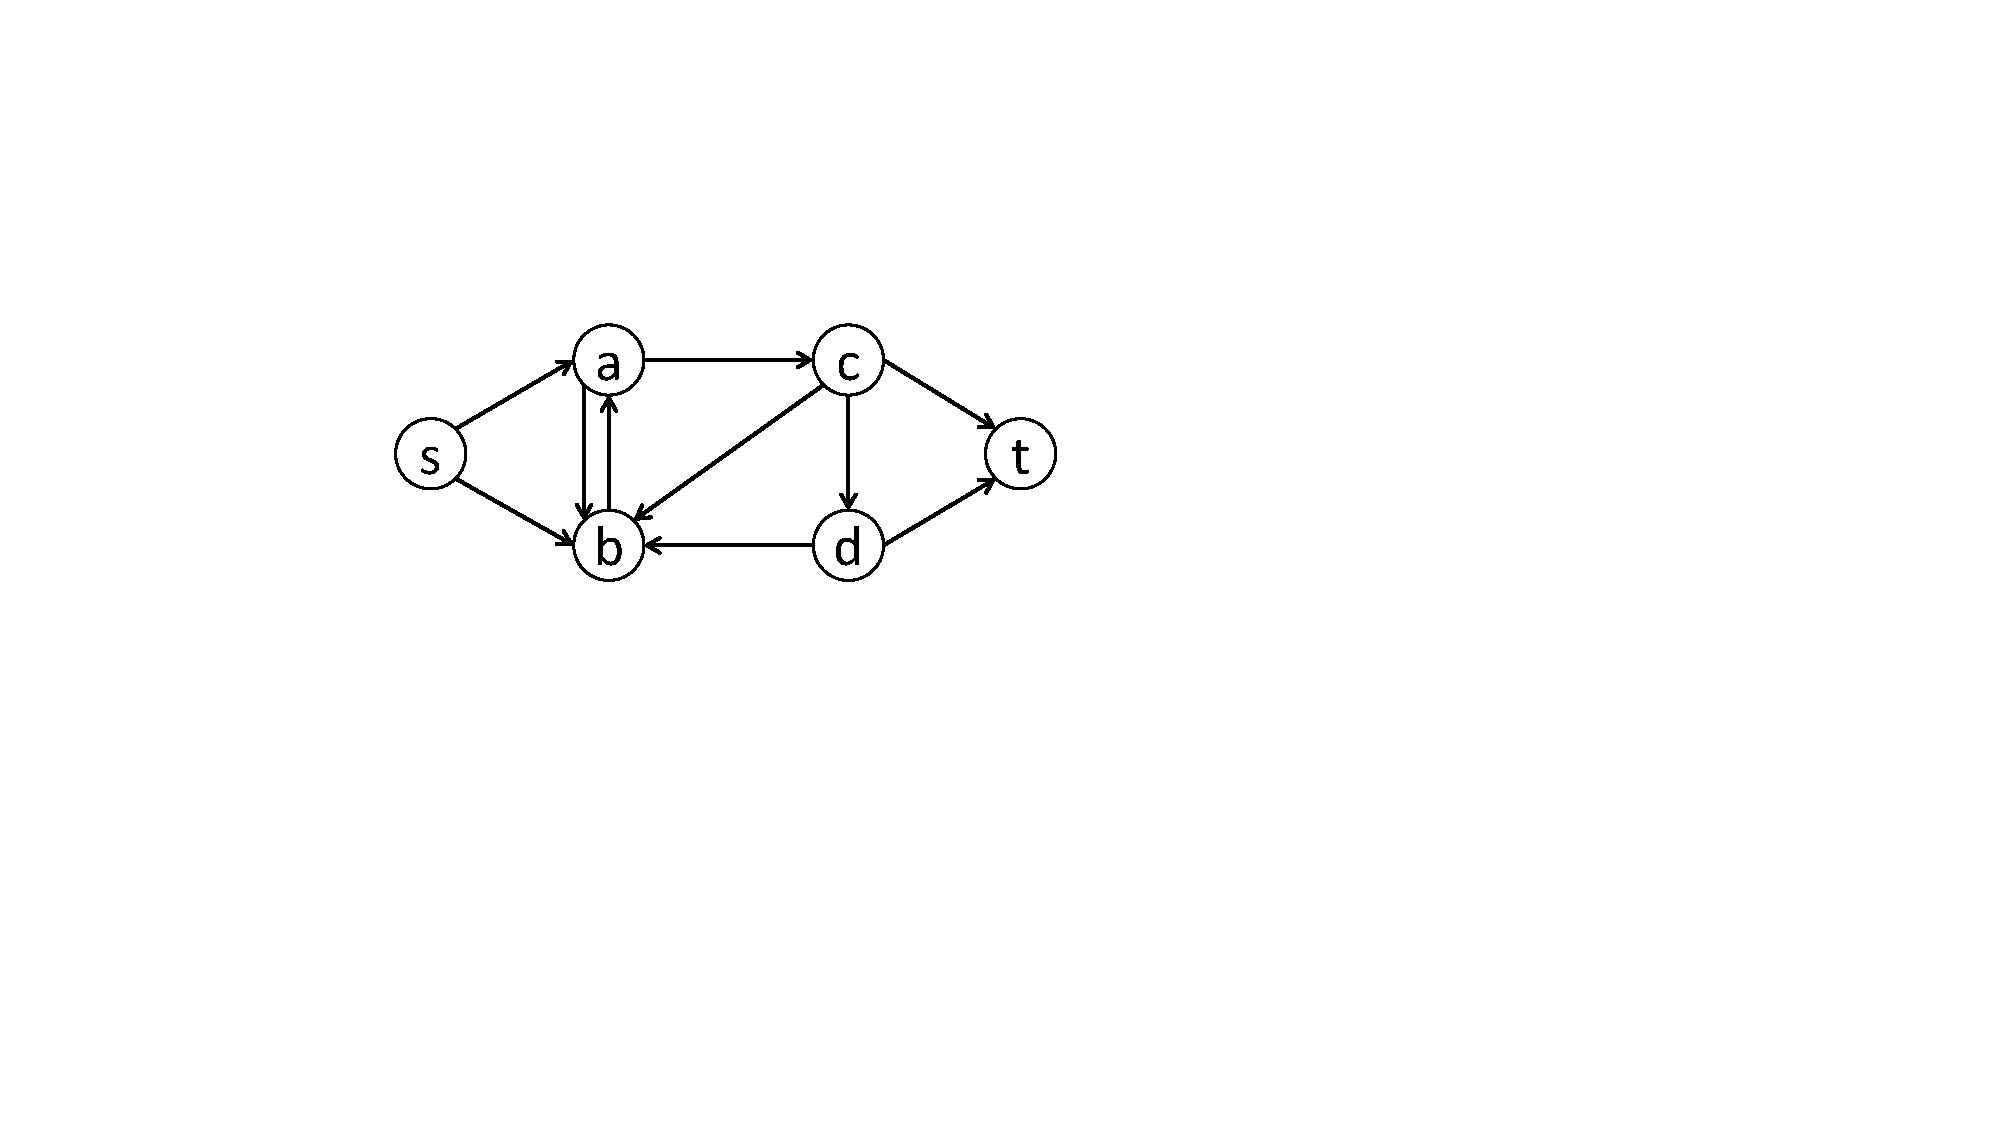
\includegraphics[width=0.7\columnwidth]{pic/graph1.pdf}
    \caption{The airline graph of a city group}
    \label{fig:graph1}
\end{figure}
To further illustrate how these methods applied with empirical data, a general setting of variables and parameters is given as follows, where $i,j$ respectively represents different city or area: 
% \begin{spacing}{1}
\begin{itemize}
    \item $c_{ij}$: the capacity of each airline from city $i$ to $j$
    
    $c_{ij} \triangleq$ $f_{ij} \cdot p_{ij}$ ($f_{ij}$: average daily flights from city $i$ to $j$; $p_{ij}$: average passenger capacity per flight. Note that $p_{ij}$ is hard to attained, and in simplified cases it's set as 1)
    
    \item $d_{ij}$: the weighted value for each airline which depends on the related demand and importance
    
    $d_{ij} \triangleq \frac{t_i}{\sum_k t_k} + \frac{g_j}{\sum_k g_k} \neq d_{ji} $ ($t_i$: total annual passenger flow of the whole airport city $i$; $g_i$: annual GDP of city $i$ ) % $D$: a normalization parameter) 
    
    \item $u_{ij}$: the utility of each airline
    $u_{ij} \triangleq c_{ij} \cdot d_{ij}$
    
    \item $S_i$: the severity of the epidemic in city $i$
    
    $S_i \triangleq I_i - E_i$ ($I_i$: average number of infections in city $i$ per day; $E_i$: average number of patients cured in city $i$ per day)
    
    \item $r_{ij}$: the rate of infection (a softmax function)
    
    $r_{ij} \triangleq e^{S_i \cdot c_{ij} / T} / (e^{S_i \cdot c_{ij} / T} + e^{S_j \cdot c_{ji} / T})$ ($T$: hyper-parameter)
    
    \item $\epsilon$: the threshold of infection rate
\end{itemize}
% \end{spacing}

Specifically, for those big cities like Beijing and Shanghai, the demand and importance of this airline $d_{ij}$ must be higher than most of cities. For different airlines, if we need to reduce the same amount for capacity $c_{ij}$, the related utility must decrease more for those airlines with higher $r_{ij}$. Thus, $u_{ij} = c_{ij} \cdot d_{ij}$ makes sense intuitively. 

Besides, the definition of $r_{ij}$ can also be explained intuitively. $r_{ij}$ is regarded as the risk of epidemic transmission, which is related to $S_i,S_j$ (the severity of the epidemic situation in the city $i,j$) and $c_{ij},c_{ji}$ (the capacity of airline $i \leftrightarrow j$). Hence, $r_{ij} = f(S_i, S_j, c_{ij}, c_{ji})$, which can be directly transformed into $r_{ij} = S_i \cdot c_{ij} / (S_i \cdot c_{ij} + S_j \cdot c_{ji})$.

To polarize the effect of $S_i \cdot c_{ij}$ and ensure the sign of $r_{ij}$ is positive (considering $S_i$ could be negative if $I_i < E_i$), we apply a softmax function $r_{ij} \triangleq e^{S_i \cdot c_{ij} / T} / (e^{S_i \cdot c_{ij} / T} + e^{S_j \cdot c_{ji} / T})$, which is the definition of $r_{ij}$. Note that the $T$ here is to adjust the polarization effect. With larger T we will have smaller polarization effect.

To derive the specific form of these variables, we need to selectively choose some datasets $\{ f_{ij},p_{ij}, I_i, E_i, t_i, g_i \}$ in real world as the basis of quantitative variables $\{ c_{ij},d_{ij}, r_{ij} \}$. 

Thus, it is natural to formulate a constrained maximization optimization problem:
\begin{align*}
    \max_{c_{ij}}~& U = \sum_{i,j} u_{ij} = \sum_{i,j} c_{ij}d_{ij}\\
    \text{subject to}~~& c_{ij} \in [0, c_{ij}^{max}],~~ \forall i \neq j \\
    & r_{ij} \le \epsilon,~~ \forall i \neq j 
\end{align*}

In order to avoid nonlinear constraints, we need to simplify the condition $r_{ij} \le \epsilon$, and then we obtain the linear constraints for $\{c_{ij}\}$:
\begin{equation*}
    \begin{aligned}
     & r_{ij} \le \epsilon,~~ \forall i \neq j \\
     \Leftrightarrow~& e^{S_i \cdot c_{ij} / T} / (e^{S_i \cdot c_{ij} / T} + e^{S_j \cdot c_{ji} / T}) \le \epsilon,~~ \forall i \neq j \\
     \Leftrightarrow~& (1-\epsilon) e^{S_i \cdot c_{ij} / T} \le \epsilon e^{S_j \cdot c_{ji} / T},~~ \forall i \neq j \\
     \Leftrightarrow~& \ln{(1-\epsilon)} + \cdot S_i \cdot c_{ij} / T \le \ln{\epsilon} + S_j \cdot c_{ji} / T,~~ \forall i \neq j \\
     \Leftrightarrow~& S_i \cdot c_{ij} - S_j \cdot c_{ji} + T \cdot \ln{\frac{1-\epsilon}{\epsilon}} \le 0,~~ \forall i \neq j
    \end{aligned}
\end{equation*}

% \textbf{Model 1: Minimum Cost Problem} 

Like fusing command by civil aviation, if the city $s$ has a serious epidemic situation, then we need to cut some airlines from the figure \ref{fig:graph1} such that
after cutting, there is no path from $s$ to $t$ (eg. capital). The cost of removing airline $i\rightarrow j$ is equal to its capacity $c_{ij}$. Thus, the problem is changed into a minimum cut problem to find a cut strategy with minimum total cost. 


% \textbf{Model 2: SI model} 

% We can choose appropriate epidemic model like SI/SIR/SIRS/SEIR models to simulate the actual situation under epidemic environment. Then rate of infection $r_{ij}$ can be described by differential equations.


% \subsection{Special Models}


\subsection{Algorithm}



\section{Performance Experiments}

We will conduct several performance experiments based on our proposed models. The quantitative analysis we may do are as follows:
\begin{itemize}
    \item To make our simulation results more representative, we will introduce several airline routes on behalf of different city scales. By collecting the number of people infected with COVID-19 and the number of susceptible and recovered people in different cities at the same time periods, we will use SI, SIR, SIRS, and SEIR models to characterize the spread of epidemics in different cities in the form of differential equations. By comparing with actual data, we will select the best-fitting infection simulation model.
    \item After obtaining the infection rate, we will determine the appropriate number of flights through the established optimization model, so as to maximize the city's utility while reducing the risk of infection as much as possible. The optimization results of different cities may vary, because the weight of routes and infection rates are different. In the most severe case of epidemic, the optimization result is likely to be a route suspension.
    \item Under the above model, we will make a decision of whether the target city will cut flights based on the current epidemic situation. By comparing with the "Five One" policy implemented by CAAC, we will analyze whether our proposed network optimization model is reasonable, and further put forward how to better formulate relevant policies through the model.
\end{itemize}

\subsection{General Settings}
We have chosen nine cities with the highest annual flight movements in 2019 and Wuhan, the pandemic center, to construct our airline network with pairwise combinations, as shown in Table 1. In particular, we only consider Beijing Capital International Airport and Shanghai Pudong International Airport since these two airports occupy more market shares in the corresponding city. 
\begin{table}[H]
    \centering
    \caption{The city group for proposed model}
    % \footnotesize
    \setlength{\tabcolsep}{1pt}
    \begin{tabular}{ccccc}
        \toprule
         1 & 2 & 3 & 4 & 5 \\
         Beijing & Shanghai & Guangzhou & Chengdu & Shenzhen \\
        \toprule
        6 & 7 & 8 & 9 & 10 \\
        Kunming & Xi'an & Chongqing & Hangzhou & Wuhan \\
        \bottomrule
    \end{tabular}
    \label{table1}
\end{table}
As mentioned in section 3.1, we need data from annual passenger flow and annual GDP to represent the weighted value of selected two city-pairs and the average number of infections and cured patients to show the rate of infections. Here we list related data for any given date in table 2. Several other statistic datasets, i.e. the maximum capacity, weighted value, severity of the epidemic and the rate of infection of the corresponding $10\times 10$ city-pairs are calculated in table 3 and table 4, shown in the appendix.

\begin{spacing}{2}
\begin{table}[H]
    \centering
    \caption{Datasets of $\{g_i, t_i, I_i, E_i\}$ (Apr. $16^{\rm th}$)}
    \setlength{\tabcolsep}{5pt}
    % \footnotesize
    \begin{tabular}{c|c|c|c|c}
        \toprule
         City $i$ & $g_i$ / trillion & $t_i$ / million & $I_i$ & $E_i$ \\
         \toprule
         1 & 3.54 & 100.2 & 593  & 50 \\
         2 & 3.82 & 76.0 & 628 & 496 \\
         3 & 2.36 & 72.7 & 499 & 449 \\
         4 & 1.70 & 55.3 & 165 & 155 \\
         5 & 2.69 & 52.3 & 459 & 429 \\
         6 & 0.65 & 48.0 & 53 & 53 \\
         7 & 0.93 & 46.9 & 120 & 117 \\
         8 & 2.36 & 44.6 & 579 & 576 \\
         9 & 1.54 & 39.8 & 181 & 181 \\
         10 & 1.62 & 26.8 & 50008 & 47283 \\
        \bottomrule
    \end{tabular}
    \label{table2}
\end{table}
\end{spacing}
In order to make our experimental results more reasonable, we have collected
the target cities' airline capacities in the past six months from Flightera\footnote{\url{https://www.flightera.net/en/}}, a website dedicating to provide accurate flight dynamic information for customers, and choose the maximum value as $c_{ij}^{max}$. As illustrated in Figure 2, we can see that there is a certain symmetry in the maximum number of flights between any two city pairs. In general, cities with more significant values have more access to other cities, as row 1 and column 1 represent the capital city Beijing. Besides, there are no flights on the diagonal since we require departure airport and destination airport are different in our model.


\begin{figure}[H]
    \centering
    \includegraphics[width=0.85\columnwidth]{pic/c_ij_max.eps}
    \caption{$c_{ij}^{max}$ from targeted city $i$ and city $j$}
    \label{fig:my_label}
\end{figure}


\subsection{Performance}
In this section, we focus on analyzing on our experimental results based on our network optimization model. In particular, we emphasize on three aspects, such as epidemic severity, the maximum airline capacity and the relaxation parameters, and analyze whether our optimized results will change when considering different modeling factors. 
\subsubsection{Relationship between $c_{ij}^* / c_{ij}^{max}$ and $S_i$}
% \begin{itemize}
%     \item Relationship between decsion making $c_{ij}^* / c_{ij}^{max}$ and the severity of epidemic $S_i$
% \end{itemize}
From section 4.1, we have given related required datasets of our model in Apr.$16^{\rm th}$. As represented in Figure 3, we regard $c_{ij}^* / c_{ij}^{max}$ as our decision variable variation. It's obvious that the more severe the pandemic in any given city becomes, the smallest airline capacity it will have. Note that there exists no flight route between Shanghai and Hangzhou, airline capacity remains zero. Without loss of generality, we consider another date which represents different levels of severity, shown in figure 3 (a). We can easily find out there are 
obvious difference in some cities less affected by the epidemic.

\begin{figure}[H]
    \centering
    \subfigure[Mar. 27$^{\rm th}$]{
        \includegraphics[width=0.46\columnwidth]{pic/decision_3-27_T_1000_ep_0dot6.eps}
    }
    \subfigure[Apr. 16$^{\rm th}$]{
        \includegraphics[width=0.46\columnwidth]{pic/decision_4-16_T_1000_ep_0dot6.eps}
    }
    \caption{Decision making $c_{ij}^* / c_{ij}^{max}$ of different date with different epidemic severity $\{S_i\}$ ($\epsilon=0.6,T=1000$)}
    \label{fig:my_label}
\end{figure}



\subsubsection{Relationship between $c_{ij}^* / c_{ij}^{max}$ and $c_{ij}^{max}$}
In section 4.2.1, we have discussed thoroughly how the parameters affect our experimental results. But there still remains a question that $c_{ij}^{max}$ in some city pairs has small value, which can impose restrictions on our optimized value to zero. With this regard, we choose two different values of $c_{ij}^{max}$ among our constructed airline network. As presented in figure 5, more proportional number of flights will be cut with higher $c_{ij}^{max}$ under the same severity of pandemic.It may Probably due to the fact that more flights can't be satisfied under this level of severity and result in smaller $c_{ij}^* / c_{ij}^{max}$.



\begin{figure}[H]
    \centering
    \subfigure[$c_{ij}^{max} = 20$]{
        \includegraphics[width=0.46\columnwidth]{pic/decision_3-27_T_1000_ep_0dot75_max_20.eps}
    }
    \subfigure[$c_{ij}^{max} = 40$]{
        \includegraphics[width=0.46\columnwidth]{pic/decision_3-27_T_1000_ep_0dot75_max_40.eps}
    }
    \caption{Decision making $c_{ij}^* / c_{ij}^{max}$ under different max capacity $c_{ij}^{max}$ on Mar. 27$^{\rm th}$ ($\epsilon=0.75,T=1000$)}
    \label{fig:my_label}
\end{figure}



\subsubsection{Relationship between $c_{ij}^* / c_{ij}^{max}$ and $c_{ij}^{max}$}
According to our proposed model, one constraint except satisfying the maximum airline capacity needs to be considered more because we aim to reduce the infection rate to an acceptable level. In this way, the threshold of infection rate $\epsilon$ and hyper-parameter $T$ should behave well to make our experimental results more practical and reasonable. In figure 4 (a) to (b), we have demonstrated the influence of parameter choices on decision variable variation in depth. In order to control covariates, we still choose Apr.$16^{\rm th}$ as the target experimental date, which represents the same level of severity. It shows that more flights will remain operational for the corresponding city pairs when we set $\epsilon$ a higher value. Comparing (a) with (e) in and (b) with (f) in figure 4 , we can conclude similarly that with larger $T$, smaller number of flights will be suspended because of the smaller effect of polarization in our constraint. Shown as before, flights remains zero in row 2 and column 9 and decision making variable of Wuhan vary small in different parameter choices.
% \begin{figure}[H]
%     \centering
%     \subfigure[$\epsilon=0.8$, $T=100$]{
%         \includegraphics[width=0.46\columnwidth]{pic/decision_4-16_T_100_ep_0.8.eps}
%     }
%     \subfigure[$\epsilon=0.9$, $T=100$]{
%         \includegraphics[width=0.46\columnwidth]{pic/decision_4-16_T_100_ep_0.9.eps}
%     }
%     \caption{Decision making $c_{ij}^* / c_{ij}^{max}$ using different $\epsilon$ on Apr. 16$^{\rm th}$}
%     \label{fig:my_label}
% \end{figure}

\begin{figure}[H]
    \centering
    \subfigure[$\epsilon=0.6$, $T=1000$]{
        \includegraphics[width=0.46\columnwidth]{pic/decision_4-16_T_1000_ep_0dot6.eps}
    }
    \subfigure[$\epsilon=0.7$, $T=1000$]{
        \includegraphics[width=0.46\columnwidth]{pic/decision_4-16_T_1000_ep_0dot7.eps}
    }
    \subfigure[$\epsilon=0.8$, $T=1000$]{
        \includegraphics[width=0.46\columnwidth]{pic/decision_4-16_T_1000_ep_0dot8.eps}
    }
    \subfigure[$\epsilon=0.9$, $T=1000$]{
        \includegraphics[width=0.46\columnwidth]{pic/decision_4-16_T_1000_ep_0dot9.eps}
    }
    \subfigure[$\epsilon=0.8$, $T=100$]{
        \includegraphics[width=0.46\columnwidth]{pic/decision_4-16_T_100_ep_0dot8.eps}
    }
    \subfigure[$\epsilon=0.9$, $T=100$]{
        \includegraphics[width=0.46\columnwidth]{pic/decision_4-16_T_100_ep_0dot9.eps}
    }
    \caption{Decision making $c_{ij}^* / c_{ij}^{max}$ using different $(\epsilon, T)$ on Apr. 16$^{\rm th}$}
    \label{fig:my_label}
\end{figure}






% \subsubsection{Relationship between decision making $c_{ij}^* / c_{ij}^{max}$ and the airline capacity $c_{ij}^{max}$}
% In section 4.2.1 and 4.2.2, we have discussed thoroughly how the parameters affect our experimental results. But there still remains a question that $c_{ij}^{max}$ in some city pairs has small value, which can impose restrictions on our optimized value to zero. With this regard, we choose two different values of $c_{ij}^{max}$ among our constructed airline network. As presented in figure 5, more proportional number of flights will be cut with higher $c_{ij}^{max}$ under the same severity of pandemic. It may Probably due to the fact that more flights can't be satisfied under this level of severity and result in smaller $c_{ij}^* / c_{ij}^{max}$.



% \begin{figure}[H]
%     \centering
%     \subfigure[$c_{ij}^{max} = 20$]{
%         \includegraphics[width=0.46\columnwidth]{pic/decision_3-27_T_1000_ep_0dot75_max_20.eps}
%     }
%     \subfigure[$c_{ij}^{max} = 40$]{
%         \includegraphics[width=0.46\columnwidth]{pic/decision_3-27_T_1000_ep_0dot75_max_40.eps}
%     }
%     \caption{Decision making $c_{ij}^* / c_{ij}^{max}$ under different max capacity $c_{ij}^{max}$ on Mar. 27$^{\rm th}$ ($\epsilon=0.75,T=1000$)}
%     \label{fig:my_label}
% \end{figure}





% \subsection{Analysis}

% \begin{itemize}
%     \item Reasonable explanation for the “Five One” policy
%     \item The impact of the severity of the epidemic $S_i$ on decision making
%     \item The impact of airline capacity $c_{ij}^{max}$ on decision making
%     \item The impact of relaxation parameters $T$ and $\epsilon$ on decision making
% \end{itemize}




% =================================


\section{Conclusion}
In this paper we focus on the assistant decision task for airline capacity control under pandemic like COVID-19. We try to model the tradeoff between the satisfaction of passengers' transportation demand and the avoidance of any further disease spreading. Our model reflects such tradeoff well and shows the difficulty of striking a balance. For getting opitmal solution we use both the IBM CPLEX solver and the Differential Evolution Algorithm, and we could get satisfactory result in the latter way. However, to answer the quesiton about anarchy penalty, that is, the negative influence of a unregulated aviation industry under global pandemic, we should further study how the capacity of aviation network could influence the infection severity in different cities with airports.

To better illustrate the relationship between decision making with different dates/cities/$\epsilon$/$T$, we also apply echarts to our Dynamic Airline System in 3D, which can be visit online\footnote{\url{demo.network-economics.whiskychoy.com}}.

From figure 7(a) and 7(b) we can see with relaxation on parameter $T$, the width of the airlines apparently increases. From figure 7(b) and figure 7(d), we know only with relaxation on parameter $T$ and lower severity at Wuhan, a small proportion of the airline capacity from Wuhan is allowed to be recovered. Finally, we also visualize the airline capacity in absolute way, that is, use $C_{ij}$ rather than $C_{ij}/C_{ij}^{max}$, and we can see from figure 7(a) and 7(c) that the actual airline capacity between cities with low $d_{ij}$ is not that large.

\begin{figure}[H]
    \centering
    \subfigure[Relative $\epsilon=.7,T=1000$]{
        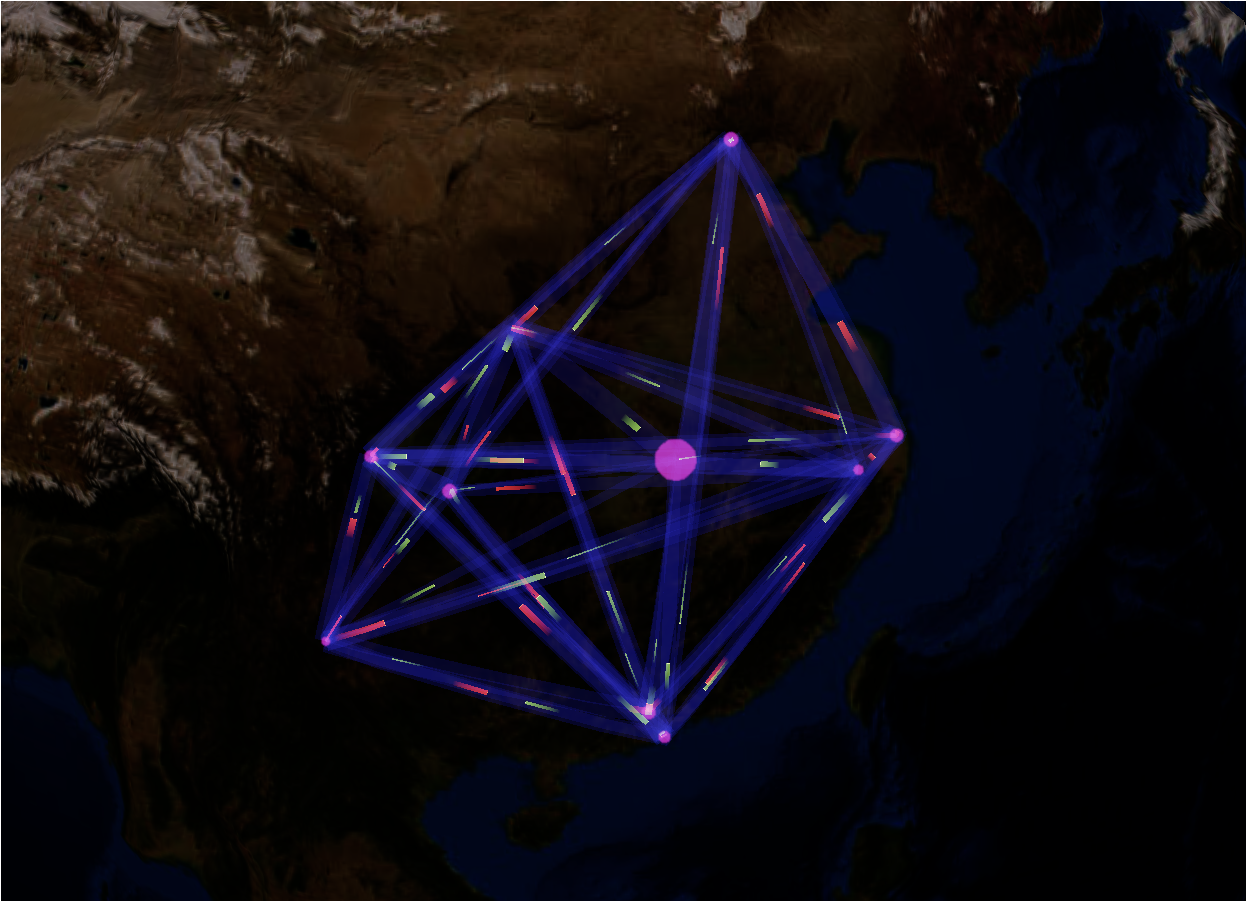
\includegraphics[width=0.46\columnwidth]{pic/relateive_T=1000_ep=0dot7_date=02162020.png}
    }
    \subfigure[Relative $\epsilon=.9, T=1000$]{
        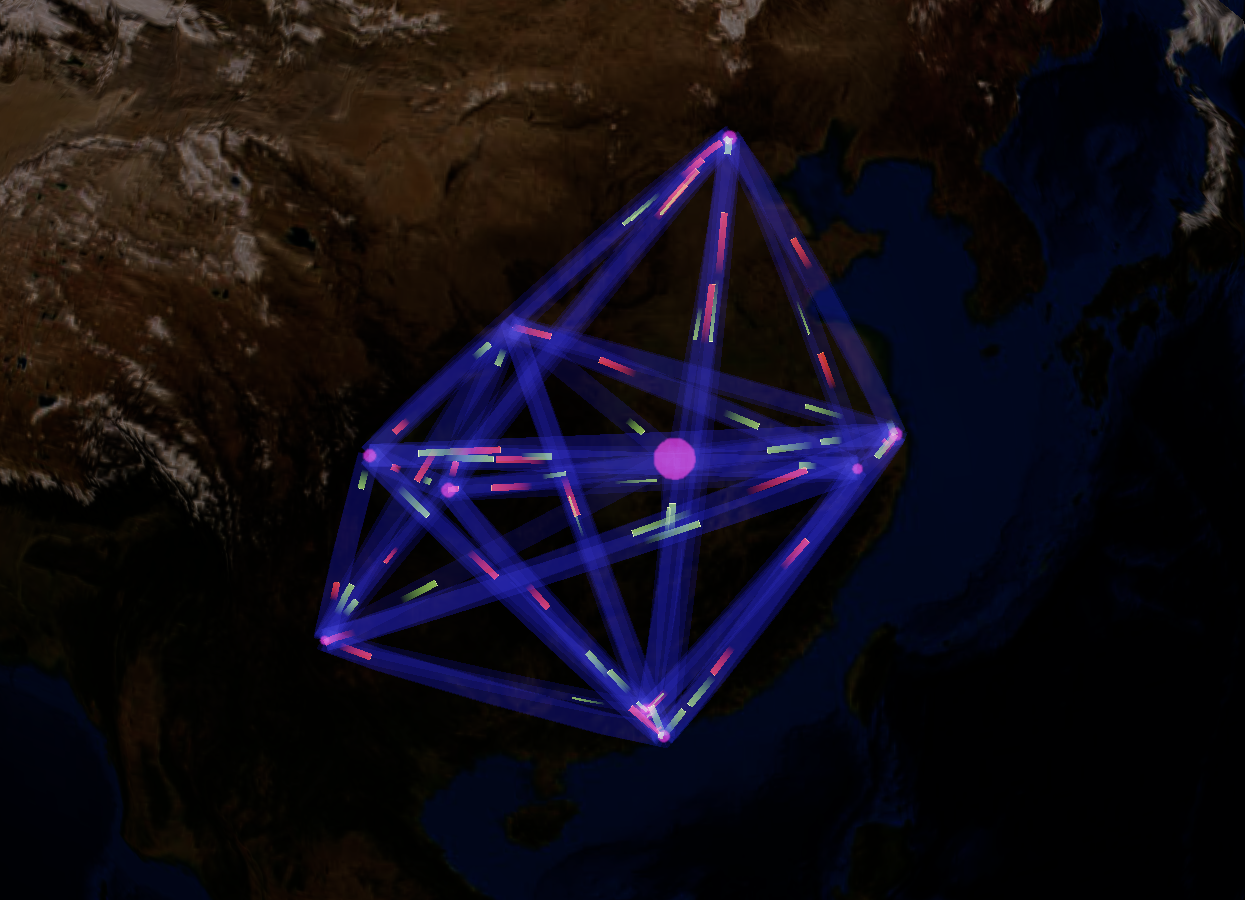
\includegraphics[width=0.46\columnwidth]{pic/relateive_T=1000_ep=0dot9_date=02162020.png}
    }
    \subfigure[Absolute $\epsilon=.7, T=1000$]{
        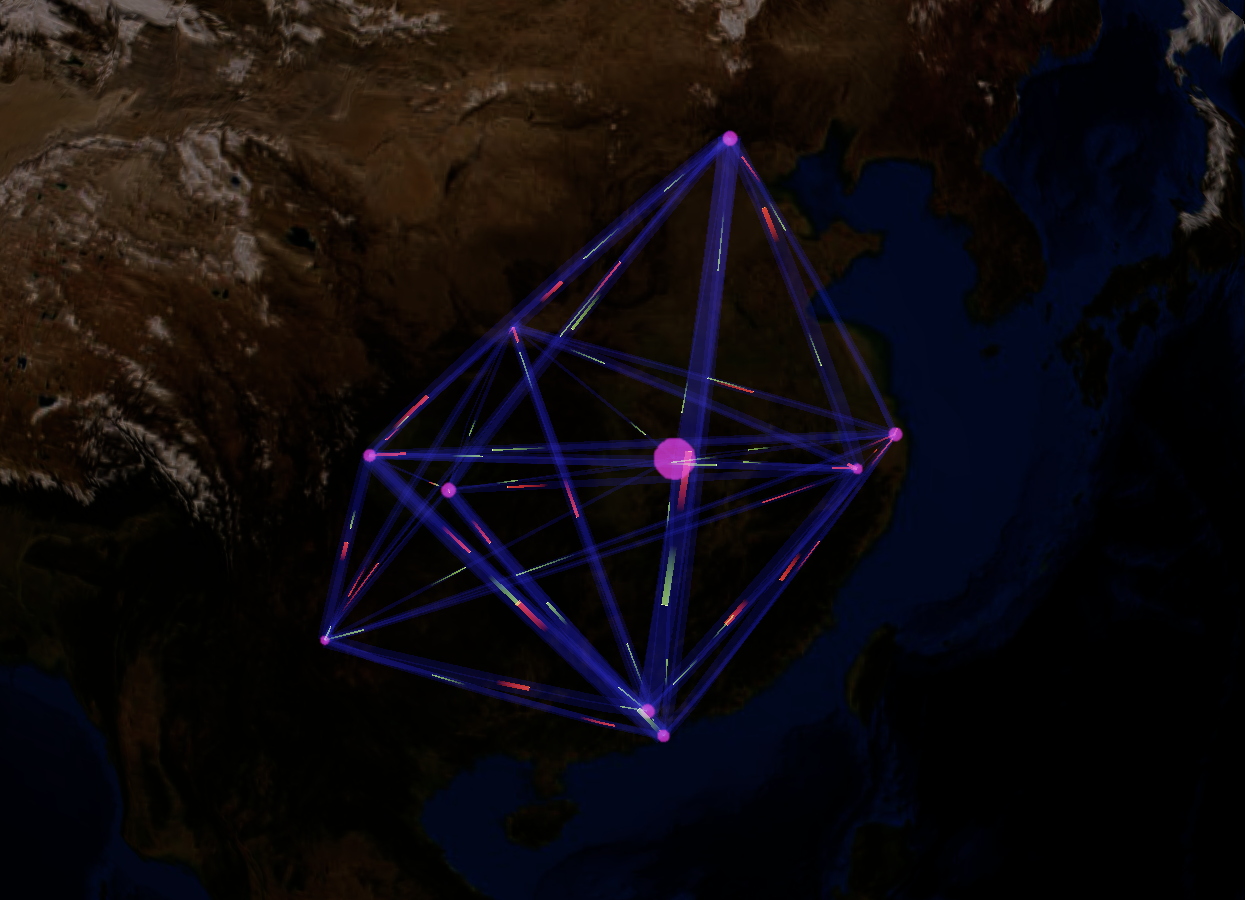
\includegraphics[width=0.46\columnwidth]{pic/absolute_T=1000_ep=0dot7_date=02162020.png}
    }
    \subfigure[Relative $\epsilon=.9, T=1000$]{
        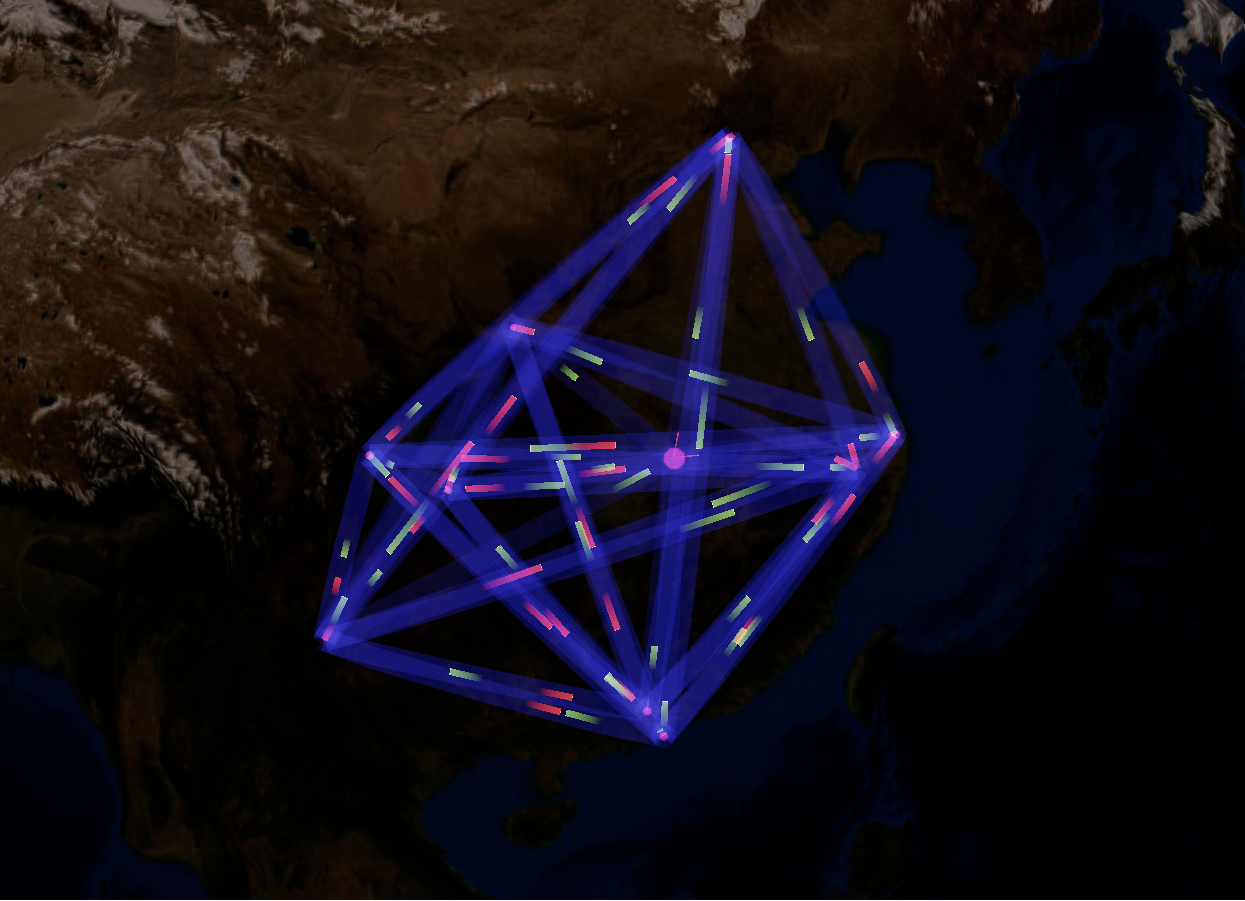
\includegraphics[width=0.46\columnwidth]{pic/relative_T=1000_ep=0dot9_date=04162020.png}
    }
    \caption{3D Airline System with Relative Capacity and Absolute Capacity. (a), (b): Feb. $16^{\rm th}$; (c), (d): Apr. $16^{\rm th}$}
    \label{fig:Convergence}
\end{figure}

% =================================
\section{Future work}

We consider



% =================================
\section{Schedule and Contribution}

In short, every small pieces of this project will be constructed by us together.
\begin{itemize}
    \item Yu Fangchen: mathmetical modeling, plot figures and writing Section 3 Proposed Model (survey of datasets $\{d_{ij}\}$) 
    \item Cai Weilin: mathmetical modeling, code writing and writing Section 1 Introduction (survey of datasets $\{c_{ij}^{max}\}$) 
    \item Li Chi: literature research, results analysis and writing Section 4 Performance Experiments (survey of datasets $\{c_{ij}^{max}\}$) 
    \item Chen Weibin: literature research and writing Section 2 Related Work (survey of datasets $\{S_i\}$) 
\end{itemize}


\bibliographystyle{unsrt}
\bibliography{refs}

% ======================

\clearpage
\section*{Appendix}

% \subsection*{Data settings}

% \begin{spacing}{1.6}
% \begin{table}[H]
%     \centering
%     \caption{Datasets of $\{g_i, t_i, I_i, E_i\}$ (Apr. $16^{\rm th}$)}
%     \setlength{\tabcolsep}{8pt}
%     % \footnotesize
%     \begin{tabular}{c|c|c|c|c}
%         \toprule
%          City $i$ & $g_i$ / trillion & $t_i$ / million & $I_i$ & $E_i$ \\
%          \toprule
%          1 & 3.54 & 100.2 & 593  & 50 \\
%          2 & 3.82 & 76.0 & 628 & 496 \\
%          3 & 2.36 & 72.7 & 579 & 576 \\
%          4 & 1.70 & 55.3 & 53 & 53 \\
%          5 & 2.69 & 52.3 & 120 & 117 \\
%          6 & 0.65 & 48.0 & 499 & 449 \\
%          7 & 0.93 & 46.9 & 181 & 181 \\
%          8 & 2.36 & 44.6 & 50008 & 47283 \\
%          9 & 1.54 & 39.8 & 459 & 429 \\
%          10 & 1.62 & 26.8 & 165 & 155 \\
%         \bottomrule
%     \end{tabular}
%     \label{table2}
% \end{table}
% \end{spacing}

% \begin{spacing}{1.6}
% \begin{table}[H]
%     \centering
%     \caption{Datasets of $\{g_i, t_i, I_i, E_i\}$}
%     % \footnotesize
%     \begin{tabular}{c|cccc}
%         \toprule
%          City $i$ & $g_i$ (Annual GDP) & $t_i$ (Annual passenger flow) & $I_i$ & $E_i$ \\
%          \toprule
%          1 &  &  &  &  \\
%          2 &  &  &  &  \\
%          3 &  &  &  &  \\
%          4 &  &  &  &  \\
%          5 &  &  &  &  \\
%          6 &  &  &  &  \\
%          7 &  &  &  &  \\
%          8 &  &  &  &  \\
%          9 &  &  &  &  \\
%          10 &  &  &  &  \\
%         \bottomrule
%     \end{tabular}
%     \label{table2}
% \end{table}
% \end{spacing}


\begin{spacing}{1.6}
\begin{table*}[btp]
    \centering
    \caption{Datasets of$\{c_{ij}^{max}\}$, $\{d_{ij}\}$ and $\{S_i(t)\}$}
    \label{table3}
    % \footnotesize 
    \setlength{\tabcolsep}{8pt}
    \renewcommand{\arraystretch}{1.2}
\begin{tabular}{c|cccccccccc}
    \toprule
    $\{c_{ij}^{max}\}$ & \multicolumn{10}{c}{City $j=1\sim10$} \\
    City $i=1\sim10$ & 1 & 2 & 3 & 4 & 5 & 6 & 7 & 8 & 9 & 10 \\ \hline
    1  &      & 9    & 30   & 32   & 33   & 18   & 21   & 23   & 28   & 13   \\
    2  & 9    &      & 9    & 18   & 12   & 10   & 15   & 18   &      & 10   \\
    3  & 30   & 10   &      & 27   & 1    & 21   & 20   & 23   & 27   & 11   \\
    4  & 33   & 18   & 27   &      & 26   & 19   & 5    & 1    & 13   & 10   \\
    5  & 34   & 12   & 2    & 26   &      & 15   & 16   & 24   & 24   & 8    \\
    6  & 18   & 9    & 20   & 19   & 14   &      & 14   & 10   & 9    & 12   \\
    7  & 21   & 14   & 21   & 5    & 16   & 13   &      & 5    & 14   & 4    \\
    8  & 23   & 19   & 23   & 2    & 24   & 10   & 5    &      & 18   & 9    \\
    9  & 28   & 1    & 27   & 13   & 25   & 9    & 14   & 18   &      & 6    \\
    10 & 14   & 9    & 11   & 10   & 8    & 12   & 4    & 9    & 6    &      \\
    \toprule
    \toprule
    $\{d_{ij}\}$ & \multicolumn{10}{c}{City $j=1\sim10$} \\
    City $i=1\sim10$ & 1 & 2 & 3 & 4 & 5 & 6 & 7 & 8 & 9 & 10 \\ \hline
    1 &  & 0.358 & 0.290 & 0.258 & 0.305 & 0.209 & 0.222 & 0.289 & 0.251 & 0.255 \\ 
    2 & 0.302 &  & 0.247 & 0.215 & 0.262 & 0.166 & 0.179 & 0.246 & 0.208 & 0.212 \\ 
    3 & 0.296 & 0.309 &  & 0.209 & 0.256 & 0.160 & 0.173 & 0.241 & 0.202 & 0.206 \\ 
    4 & 0.265 & 0.278 & 0.210 &  & 0.225 & 0.129 & 0.142 & 0.210 & 0.171 & 0.175 \\ 
    5 & 0.260 & 0.273 & 0.204 & 0.173 &  & 0.124 & 0.137 & 0.204 & 0.165 & 0.169 \\ 
    6 & 0.252 & 0.265 & 0.197 & 0.166 & 0.212 &  & 0.129 & 0.197 & 0.158 & 0.162 \\ 
    7 & 0.250 & 0.263 & 0.195 & 0.164 & 0.210 & 0.114 &  & 0.195 & 0.156 & 0.160 \\ 
    8 & 0.246 & 0.259 & 0.191 & 0.159 & 0.206 & 0.110 & 0.123 &  & 0.152 & 0.156 \\ 
    9 & 0.237 & 0.251 & 0.182 & 0.151 & 0.198 & 0.101 & 0.115 & 0.182 &  & 0.147 \\ 
    10 & 0.214 & 0.228 & 0.159 & 0.128 & 0.175 & 0.078 & 0.092 & 0.159 & 0.120 &  \\ 
    \toprule
    \toprule
    $\{S_{i}(t)\}$ & \multicolumn{10}{c}{Date $t$: Feb. 16$^{\rm th}$ $\sim$ Apr. 16$^{\rm th}$} \\
    City $i=1\sim10$ & 1 & 2 & 3 & 4 & 5 & 6 & 7 & 8 & 9 & 10 \\ \hline
    Feb 16 & 263 & 190 & 287 & 87 & 80 & 2 & 0 & 339 & 12 & 37692   \\ 
    Feb 22 & 206 & 105 & 271 & 84 & 196 & 23 & 18 & 239 & 95 & 38450 \\ 
    Feb 29 & 129 & 47 & 264 & 80 & 278 & 36 & 65 & 132 & 141 & 34437 \\ 
    Mar 06 & 115 & 33 & 237 & 62 & 298 & 30 & 95 & 44 & 109 & 29895 \\ 
    Mar 16 & 79 & 30 & 189 & 43 & 232 & 0 & 82 & 0 & 74 & 19935 \\ 
    Mar 22 & 114 & 72 & 154 & 23 & 158 & 0 & 76 & 1 & 48 & 16861 \\ 
    Mar 28 & 157 & 153 & 144 & 4 & 100 & 0 & 46 & 3 & 30 & 9973 \\ 
    Apr 03 & 139 & 175 & 140 & 12 & 70 & 0 & 30 & 3 & 5 & 4588 \\ 
    Apr 10 & 107 & 113 & 129 & 19 & 49 & 0 & 19 & 3 & 2 & 3145 \\ 
    Apr 16 & 76 & 132 & 50 & 10 & 30 & 0 & 3 & 3 & 0 & 2725 \\ 
    \bottomrule
\end{tabular}
\end{table*}
\end{spacing}

% \begin{spacing}{1.6}
% \begin{table*}[btp]
%     \centering
%     \caption{Results of$\{r_{ij}\}$ (eg. Apr. 16$^{\rm th}$)}
%     \label{table3}
%     % \footnotesize 
%     \setlength{\tabcolsep}{8pt}
%     \renewcommand{\arraystretch}{1.2}
% \begin{tabular}{c|cccccccccc}
%     \toprule
%     $\{r_{ij}\}$ & \multicolumn{10}{c}{City $j=1\sim10$} \\
%     City $i=1\sim10$ & 1 & 2 & 3 & 4 & 5 & 6 & 7 & 8 & 9 & 10 \\ \hline
%     1 &  &  &  &  &  &  &  &  &  &  \\ 
%     2 &  &  &  &  &  &  &  &  &  &  \\ 
%     3 &  &  &  &  &  &  &  &  &  &  \\ 
%     4 &  &  &  &  &  &  &  &  &  &  \\ 
%     5 &  &  &  &  &  &  &  &  &  &  \\ 
%     6 &  &  &  &  &  &  &  &  &  &  \\ 
%     7 &  &  &  &  &  &  &  &  &  &  \\ 
%     8 &  &  &  &  &  &  &  &  &  &  \\ 
%     9 &  &  &  &  &  &  &  &  &  &  \\ 
%     10 &  &  &  &  &  &  &  &  &  &  \\ 
%     \bottomrule
% \end{tabular}
% \end{table*}
% \end{spacing}


\end{document}
